\documentclass{beamer} 
\usepackage[utf8]{inputenc}
\usepackage{multicol}
\usepackage{url}
\usepackage{fancyvrb}
\usepackage{color}
\setbeamercolor{goodcolor}{fg=black,bg=lime}
\setbeamercolor{badcolor}{fg=black,bg=pink}

\title{What every programmer should know about merging branches in Mercurial} 
\author{Sergey Kishchenko} 
\date{\today} 
\usetheme{CambridgeUS}
\usecolortheme{seagull}
\institute{Quickoffice}

\begin{document}

\frame{\titlepage}

\begin{frame} 
\frametitle{Branches}
\begin{multicols}{2}
\center{Two different branches}
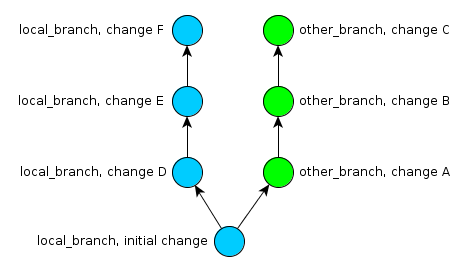
\includegraphics[width=0.4\textwidth]{img/two_branches}
\columnbreak
\center{Two different defaults}
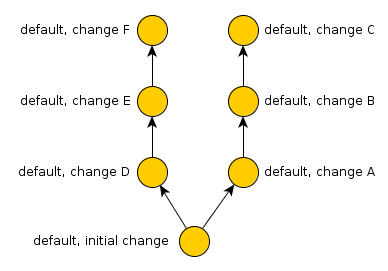
\includegraphics[width=0.4\textwidth]{img/two_default_branches}
\end{multicols}
\begin{itemize}
\item \textbf{NOTE}: Different repos cloned from one source are not actually different, they are more like one repo. You can transfer changes between them with push and pull
\item \textbf{IMPORTANT}: Named branches in Mercurial are permanent!
\end{itemize}
\end{frame}

\begin{frame}[fragile]
\frametitle{Pull}
\begin{exampleblock}{First step in merge process: pulling remote changes}
\begin{verbatim}
> hg pull -b REMOTE_BRANCH REMOTE_REPO
\end{verbatim}
\end{exampleblock}
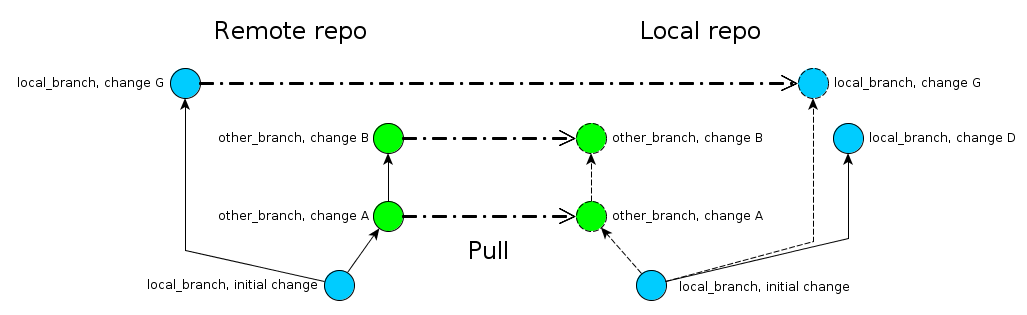
\includegraphics[width=\textwidth]{img/pull_branches}
\begin{itemize}
\item Pulling change pulls also all its ancestors $\to$ unneeded changes
\item Pulling changes may result in creating new heads $\to$ merge is needed
\end{itemize}
\end{frame}

\begin{frame}
\frametitle{Solution attempt: "early-fix" branch}
\begin{multicols}{2}
\center{Bad idea}
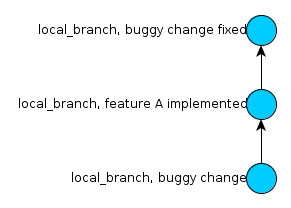
\includegraphics[width=0.4\textwidth]{img/early_fix_branch_bad}
\columnbreak
\center{Good idea}
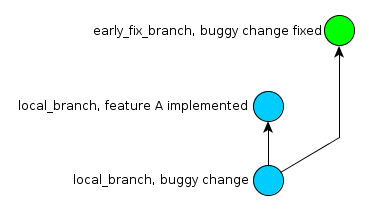
\includegraphics[width=0.4\textwidth]{img/early_fix_branch_good}
\end{multicols}
\begin{beamercolorbox}[rounded=true,center,shadow=true]{goodcolor}
  Having a specific fix branch allows pulling this branch without pulling other changes (Feature A)
\end{beamercolorbox}
\begin{beamercolorbox}[rounded=true,center,shadow=true]{badcolor}
  You should think about it in advance and you're not a psychic
\end{beamercolorbox}
\end{frame}

\begin{frame}
\frametitle{Solution attempt: Patch}
\textbf{IDEA}: Why do we even need to use pull?
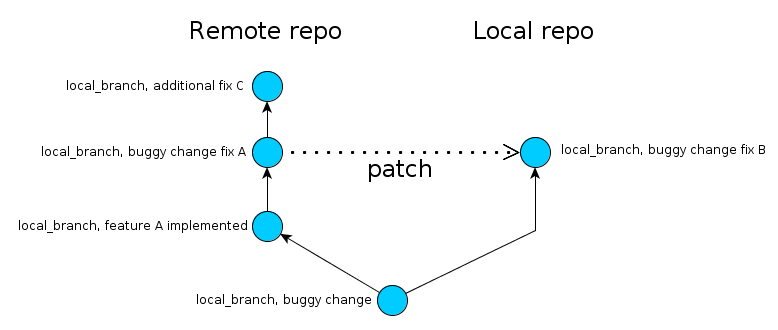
\includegraphics[width=\textwidth]{img/using_patch}

\begin{beamercolorbox}[rounded=true,center,shadow=true]{badcolor}
  Fix A can be based on Feature A so patch will not apply smoothly
\end{beamercolorbox}
\begin{beamercolorbox}[rounded=true,center,shadow=true]{badcolor}
  SCM can't guess that fix A and fix B are actually the same and should be used as base when merging fix C
\end{beamercolorbox}
\end{frame}

\begin{frame}[fragile]
\frametitle{Solution attempt: graft}
\begin{exampleblock}{Using graft}
\begin{verbatim}
> hg graft --log GRAFT_REVISION
\end{verbatim}
\end{exampleblock}
\begin{center}
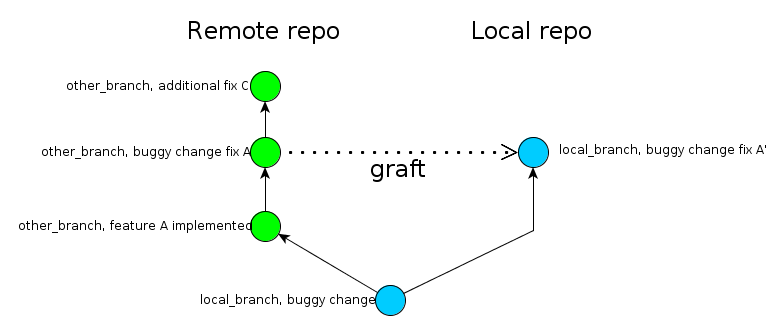
\includegraphics[width=0.8\textwidth]{img/using_graft}
\end{center}

\begin{beamercolorbox}[rounded=true,center,shadow=true]{goodcolor}
  graft uses 3-way merge and deals fine with Fix A being based on Feature A
\end{beamercolorbox}
\begin{beamercolorbox}[rounded=true,center,shadow=true]{badcolor}
  SCM still can't guess that fix A and fix B are actually the same and should be used as base when merging fix C
\end{beamercolorbox}
\end{frame}

\begin{frame}[fragile]
\frametitle{Solution attempt: grafting from remote repo}
\textit{hg graft} doesn't deal with changesets from the remote repo at the moment because it needs all of the changes to do 3-way merge. But it's possible to strip changes when they are not needed anymore
\begin{exampleblock}{grafting from remote repository}
\begin{verbatim}
> hg incoming --template="{node} " REMOTE_REPO -q \ 
    -r GRAFT_REVISION > TEMP_FILE
> hg pull -r GRAFT_REVISION REMOTE_REPO
> hg graft --log GRAFT_REVISION
> hg strip `cat TEMP_FILE`
\end{verbatim}
\end{exampleblock}
\end{frame}

\begin{frame}
\frametitle{Solution attempt: dealing with base issues with graft}
\begin{center}
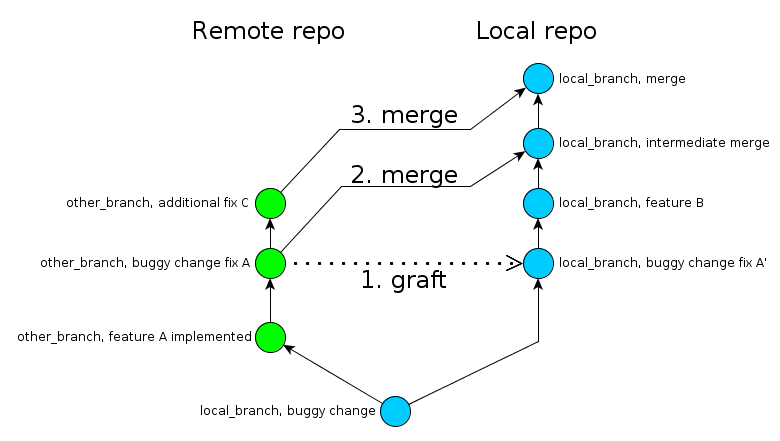
\includegraphics[width=\textwidth]{img/graft_dealing_with_base}
\end{center}
\end{frame}

\begin{frame}[fragile]
\frametitle{Solution attempt: dealing with base issues with graft}
\begin{exampleblock}{Searching for grafted revisions}
\begin{Verbatim}[fontsize=\small]
> hg log -r "ancestor(LOCAL_HEAD,OTHER_HEAD)::LOCAL_HEAD" \
    -k "grafted" -v
e.g.
> hg log -r "ancestor(d5c1ff557965,927d19ecf38e)::d5c1ff557965" \
    -k "grafted" -v
\end{Verbatim}
\end{exampleblock}

\begin{exampleblock}{graft-aware merging}
\begin{verbatim}
> hg merge -R GRAFT_REVISION
> hg merge
\end{verbatim}
\end{exampleblock}
\end{frame}

\begin{frame} 
\frametitle{Solution attempt: Branches alternatives}
\begin{itemize}
\item Bookmarks: \url{http://mercurial.selenic.com/wiki/Bookmarks}
\begin{beamercolorbox}[rounded=true,center,shadow=true, wd=0.9\textwidth]{goodcolor}
Lightweight git-like branches, good for local hacking, distributed along with Mercurial. 
\end{beamercolorbox}
\begin{beamercolorbox}[rounded=true,center,shadow=true, wd=0.9\textwidth]{badcolor}
Several heads on default, no trail in history
\end{beamercolorbox}
\item Local branches, lbranches: \url{http://mercurial.selenic.com/wiki/LocalbranchExtension}. 
\begin{beamercolorbox}[rounded=true,center,shadow=true, wd=0.9\textwidth]{goodcolor}
Lightweight repo clones, good for local hacking
\end{beamercolorbox}
\begin{beamercolorbox}[rounded=true,center,shadow=true, wd=0.9\textwidth]{badcolor}
Just a local feature
\end{beamercolorbox}
\item Patch queues, mq: \url{http://mercurial.selenic.com/wiki/MqExtension} 
\begin{beamercolorbox}[rounded=true,center,shadow=true, wd=0.9\textwidth]{goodcolor}
Patch series, editable history, distributed along with Mercurial
\end{beamercolorbox}
\begin{beamercolorbox}[rounded=true,center,shadow=true, wd=0.9\textwidth]{badcolor}
Just a local feature
\end{beamercolorbox}
\end{itemize}
\end{frame}


\begin{frame}[fragile]
\frametitle{Merge}
\begin{columns}[T]
\begin{column}{0.45\textwidth}
\begin{exampleblock}{Merging default branches}
\begin{verbatim}
> hg co local_branch
> hg merge remote_branch
\end{verbatim}
\end{exampleblock}
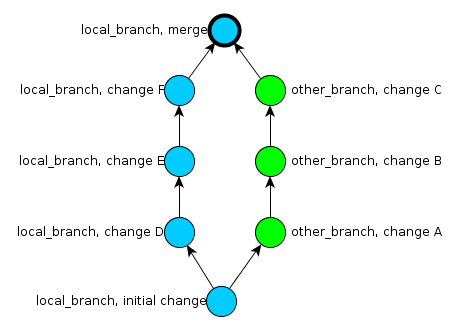
\includegraphics[width=\textwidth]{img/two_branches_merged}
\end{column}

\begin{column}{0.45\textwidth}
\begin{exampleblock}{Merging heads in default}
\begin{verbatim}
> hg merge 
(while in default)
\end{verbatim}
\end{exampleblock}
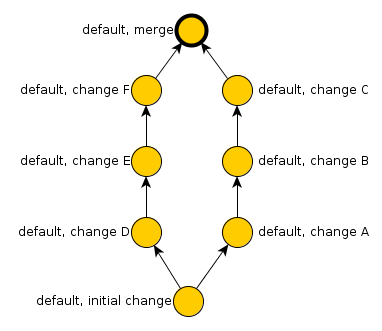
\includegraphics[width=0.86\textwidth]{img/two_default_branches_merged}
\end{column}
\end{columns}
\begin{center}
It isn't always so good :( 
\end{center}
\end{frame}

\begin{frame}
\frametitle{Merge problem: too much conflicts}
\begin{itemize}
\item \textbf{Why occurs?}
\begin{itemize}
\item Synchronizing rarely
\item Tight coupling of the components
\item Too many developers for one component
\end{itemize}
\item \textbf{How to prevent?}
\begin{itemize}
\item Synchronize often
\item Simplify connections between components
\item Design clear and minimalistic API
\item Notify other developers of the component when doing changes
\item Don't exceed the reasonable amount of developers on one component 
\end{itemize}
\item \textbf{How to deal with?}
\begin{itemize}
\item Use a good graphical merge tool that allows 3-way merging
\item Learn how to use the \textit{resolve} command
\end{itemize}
\end{itemize}
\end{frame}

\begin{frame}[fragile]
\frametitle{3-way merge}
\begin{columns}[T]
\begin{column}{0.45\textwidth}
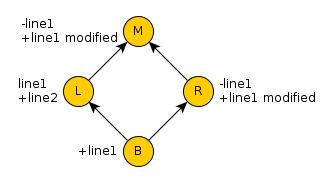
\includegraphics[width=\textwidth]{img/3way_merge}

\begin{exampleblock}{Merged (M)}
\begin{verbatim}
line1 modified
line2
\end{verbatim}
\end{exampleblock}

\end{column}
\begin{column}{0.45\textwidth}
\begin{exampleblock}{Base (B)}
\begin{verbatim}
line1
\end{verbatim}
\end{exampleblock}

\begin{exampleblock}{Local (L)}
\begin{verbatim}
line1
line2
\end{verbatim}
\end{exampleblock}

\begin{exampleblock}{Remote (R)}
\begin{verbatim}
line1 modified
\end{verbatim}
\end{exampleblock}

\end{column}
\end{columns}

\begin{center}
Without base it's hard to merge Local and Remote files: it's hard to understand was it a removal of "line2" and addition of " modified" or removal of " modified" and addition of "line2" $\to$ use a 3-way graphical merge tool
Subjective choice: \url{http://mercurial.selenic.com/wiki/KDiff3}
\end{center}
\end{frame}

\begin{frame}[fragile]
\frametitle{\textit{resolve} command}
Imagine you need to merge \textbf{a lot} of changes

\begin{exampleblock}{Bad idea}
\begin{verbatim}
> hg merge # non-stop merging, here I come!
\end{verbatim}
\end{exampleblock}

\begin{exampleblock}{Good idea}
\begin{Verbatim}[fontsize=\footnotesize]
> hg merge -t "internal:merge" # does the best it can automatically
> hg resolve -l # shows merge state
> hg resolve FILE # runs conflict resolving for specific files
> hg resolve -a # runs conflict resolving for all unresolved files
\end{Verbatim}
\end{exampleblock}
\textbf{IMPORTANT}: Unfortunately, \textit{resolve} command doesn't save progress when interrupted. There is an issue for that: \url{http://bz.selenic.com/show_bug.cgi?id=3638}. 

Possible workaround: iterate through conflicts and call \textit{resolve} for each file
\end{frame}

\begin{frame}
\frametitle{Merge problem: hard to understand the conflict}
Also known as "I don't know which change is correct"


\begin{itemize}
\item \textbf{Why occurs?}
\begin{itemize}
\item Synchronizing rarely $\to$ forgetting what was going on
\item Merging components without component knowledge
\end{itemize}
\item \textbf{How to prevent?}
\begin{itemize}
\item Synchronize often
\item Spread the components knowledge among developers $\to$ code cross-review
\end{itemize}
\item \textbf{How to deal with?}
\begin{itemize}
\item Use help from those who have good component knowledge
\item Learn how to use \textit{log} (shows the history) and \textit{blame} (shows who is the author of the changes) command
\end{itemize}
\end{itemize}
\end{frame}

\begin{frame}
\frametitle{Merge problem: code was refactored}
Also known as "It seems the code was removed remotely so I can drop the local change" (immediately eaten by velociraptor)


\begin{itemize}
\item \textbf{Why occurs?}
\begin{itemize}
\item Doing the refactoring and not merging it into all branches immediately
\item Merging refactored components without component knowledge
\end{itemize}
\item \textbf{How to prevent?}
\begin{itemize}
\item Spread the components knowledge among developers $\to$ code cross-review
\item Use "early-fix" branches for refactoring and merge them immediately
\end{itemize}
\item \textbf{How to deal with?}
\begin{itemize}
\item Use help from those who have good knowledge about the refactoring
\item In case different refactoring was done in both local and remote versions, you're DOOMed :(
\item Use 3-way merge (check next slide)
\end{itemize}
\end{itemize}
\end{frame}

\begin{frame}[fragile]
\frametitle{Using 3-way merge for merging refactored code}
\begin{enumerate}
\item Use 3-way merge graphical tool to see base(B), local(L) and remote(R) version of a file
\item Let's assume refactoring was done only in remote. It means that base-local difference is not large, it's all about modifying names, adding params, issues fix, etc. Base and remote differ a lot, often the remote version is completely missing, i.e., was moved to different file.
\item Use \textit{log} to identify what was refactoring about. E.g., you can find the file that is a new home for code that is missing from the R
\begin{exampleblock}{Use \textit{log} to find refactoring changesets}
\begin{verbatim}
> hg log --removed --follow R 
\end{verbatim}
\end{exampleblock}
\item Iterate through base-local differences change-by-change and apply them to the code in a correct-place
\item In any case consider contacting those who did the refactoring for help and/or code review
\end{enumerate}
\end{frame}

\begin{frame}
\frametitle{Non-source files conflicts}
TODO: Why occurs? How to prevent? How to deal with? 
\end{frame}


\begin{frame}
\frametitle{One more time: good things}
\begin{itemize}
\item Specifying branch for pulling
\item Using graft
\item Using good graphical tool for merging
\item Using 3-way merge
\item Using "early-fix" branches
\item Getting knowledge from others when merging theirs code
\item Providing help to those who merge your code
\end{itemize}
\end{frame}

\begin{frame}
\frametitle{One more time: bad things}
\begin{itemize}
\item Manual merges
\item Applying patches manually
\item Being a coward and selecting one side
\item Trusting automatic merge tools completely
\end{itemize}
\end{frame}

\begin{frame}
\frametitle{One more time: things to avoid}
\begin{itemize}
\item Doing a refactoring that can't be merged into all branches immediately
\item Modifying non-source file without merging it into all branches immediately
\item Modifying a component that somebody is working on without notifying him 
\end{itemize}
\end{frame}


\begin{frame}
\frametitle{Thank you! Questions?}
\begin{center}
% \includegraphics[width=0.45\textwidth]{img/chubaka}
\end{center}
\end{frame}

\end{document}
